\documentclass{standalone}
\usepackage{pgfplots}
\pgfplotsset{compat=1.18}

\begin{document}

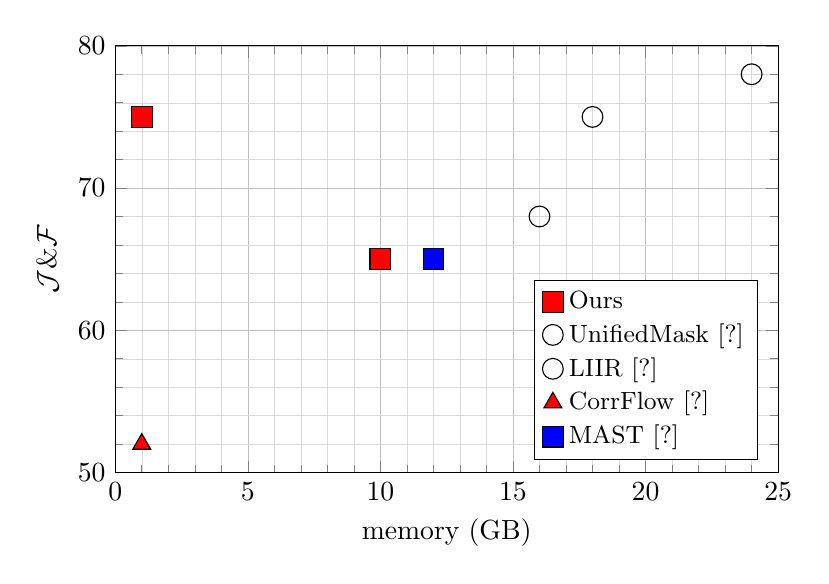
\begin{tikzpicture}
    \begin{axis}[
        width=10cm,
        height=7cm,
        xlabel={memory (GB)},
        ylabel={$\mathcal{J}\&\mathcal{F}$},
        xmin=0, xmax=25,
        ymin=50, ymax=80,
        xtick={0,5,10,15,20,25},
        ytick={50,60,70,80},
        grid=both,
        grid style={line width=.1pt, draw=gray!30},
        major grid style={line width=.2pt,draw=gray!50},
        minor tick num=4,
        legend pos=south east,
        legend cell align={left},
        legend style={
            font=\small,
            /tikz/every even column/.append style={column sep=5pt}
        }
    ]

    % Data for "Ours" (red square)
    \addplot[
        only marks,
        mark=square*,
        mark options={fill=red, scale=1.5},
        mark size=2.5pt
    ] coordinates {
        (1, 75) % Example data point
        (10, 65) % Example data point
    };
    \addlegendentry{Ours};

    % Data for "UnifiedMask [?]" (circle)
    \addplot[
        only marks,
        mark=o,
        mark options={scale=1.5},
        mark size=2.5pt
    ] coordinates {
        (18, 75) % Example data point
        (24, 78) % Example data point
    };
    \addlegendentry{UnifiedMask [?]};

    % Data for "LIIR [?]" (circle)
    \addplot[
        only marks,
        mark=o,
        mark options={scale=1.5},
        mark size=2.5pt
    ] coordinates {
        (16, 68) % Example data point
    };
    \addlegendentry{LIIR [?]};

    % Data for "CorrFlow [?]" (triangle)
    \addplot[
        only marks,
        mark=triangle*,
        mark options={fill=red, scale=1.5},
        mark size=2.5pt
    ] coordinates {
        (1, 52) % Example data point
    };
    \addlegendentry{CorrFlow [?]};

    % Data for "MAST [?]" (square)
    \addplot[
        only marks,
        mark=square*,
        mark options={fill=blue, scale=1.5},
        mark size=2.5pt
    ] coordinates {
        (12, 65) % Example data point
    };
    \addlegendentry{MAST [?]};

    \end{axis}
\end{tikzpicture}

\end{document}